Der im Kapitel \ref{chap:loesungsansatz} erarbeitete Lösungsansatz soll nun
in einem ``Proof of Concept'' anhand einem realen Projekt durchgespielt und getestet
werden.

Der Studierende ist in der glücklichen Lage, dass allink zum Zeitpunkt der
Erstellung dieses ``Proof of Concepts'' über ein noch nicht gestartetes Projekt 
mit Abgabetermin 27. Mai 2011 verfügt. Dieses Projekt wird nun anhand dem neuen
Projektablauf durchgespielt und dabei alle definierten Instrumente verwendet.

Bei der nachfolgenden Beschreibung des realen Projektverlaufes wird jeweils auf
die einzelnen Schritte des definierten Projektverlaufes des Lösungsansatzes
verwiesen. An den jeweiligen Stellen wo Instrumente zum Einsatz kommen, werden
diese mit Hilfe von Screenshots dargestellt.

\section{Projektdefinition}
Der Kunde Reisana\footnote{Der Name des Kunden wurde absichtlich geändert, da
allink den Kunden nicht explizit in dieser Arbeit erwähnt haben möchte.} ist aufgrund 
einer Empfehlung auf allink zugegangen und möchte (\textbf{0}), dass sie für ihn 
einen Facebook Wettbewerb umsetzen. Die Anfrage wurde von den Partner diskutiert 
(\textbf{1.1}) und angenommen (\textbf{1.2}).

Als verantwortlicher Partner wurde Silvan Spross definiert. Er übernimmt
zugleich auch die Projektleitung, da es ein eher kleines Projekt ist und dazu
nicht zwingend noch eine zusätzliche Person benötigt wird (\textbf{3.1}). Der 
Projektleiter hat darauf den, in der nachstehenden Tabelle \ref{tab:projektbrief_poc} dargestellte,
Projektbrief (\textbf{3.2}) erstellt.

\begin{longtable}{lp{10cm}}
    \toprule \textbf{Element} & \textbf{Beschreibung} \\
    \midrule Kunde, Kontaktperson &
        Reisana, Hans Muster\footnote{Auch hier wurde der Name der Kontaktperson
        absichtlich geändert.} \\
    \midrule Projekt &
        Reisana Facebook Wettbewerb \\
    \midrule Datum &
        23. Mai 2011 \\
    \midrule Hintergrund &
        Reisana ist ein Reisebüro. Sie möchten über Facebook einen Fotowettbewerb
        veranstalten, wo die Teilnehmer mit Hilfe der Stimmen ihrer Freunde 
        Reisegutscheine gewinnen können. \\
    \midrule Aufgabe &
        allink soll einen Facebook Wettbewerb erstellen, wo die Teilnehmer mit
        ihrem Facebookprofil Fotos hochladen können. Sie selbst, ihre Freunde
        und andere Facebook Benutzer können dann für die Fotos ihre Stimme abgeben.
        Nach einem gewissen Zeitraum gewinnen die Teilnehmer mit den meisten 
        Stimmen Gutscheine im Wert von 500.- bis 1'000.- CHF. \\
    \midrule Ziel &
        Es soll ein gut funktionierender Wettbwerb erstellt werden, der einfach
        zu bedienen. Zusätzlich sollen die Likes für die Facebookprofilseite von
        Reisana erhöht werden. \\
    \midrule Zielgruppe &
        Die Zielgruppe sind Facebookuser mit dem Alter ab 18 Jahren. \\
    \midrule Botschaft und USP &
        Der Facebookwettbewerb muss sauber in die Facebookumgebung integriert 
        sein, damit die Bereitschaft der Teilnehmer hoch ist. \\
    \midrule Tonalität &
        Da Facebook überwiegend von jüngeren Menschen benutzt wird, wird die
        Bild- und Textsprache jung und fancy sein. \\
    \midrule Vorgaben, Obligatorisches &
        Das Logo von Reisana und ihre Keyvisuals müssen verwendet werden. \\
    \bottomrule
    \caption[Projektbrief des Facebookwettbewerbs für Hotelplan]{Projektbrief des 
        Facebookwettbewerbs für Hotelplan\footnotemark}
    \label{tab:projektbrief_poc}
\end{longtable}
\footnotetext{Eigene Darstellung}

Nach der Erstellung des Projektbriefs weiss der Projektleiter, dass er mindestens
einen Grafiker und einen Entwickler für das Projekt benötigt. Die Wahl fällt
auf diejenigen Mitarbeiter, die bereits bei einem ähnlichen Facebookwettbewerb
mitgearbeitet haben (\textbf{3.2}). In der nachfolgenden Grafik \ref{pic:projektorganisation_poc} 
ist der Aufbau der Projektorganisation ersichtlich.

\begin{figure}[htbp]
\begin{center}
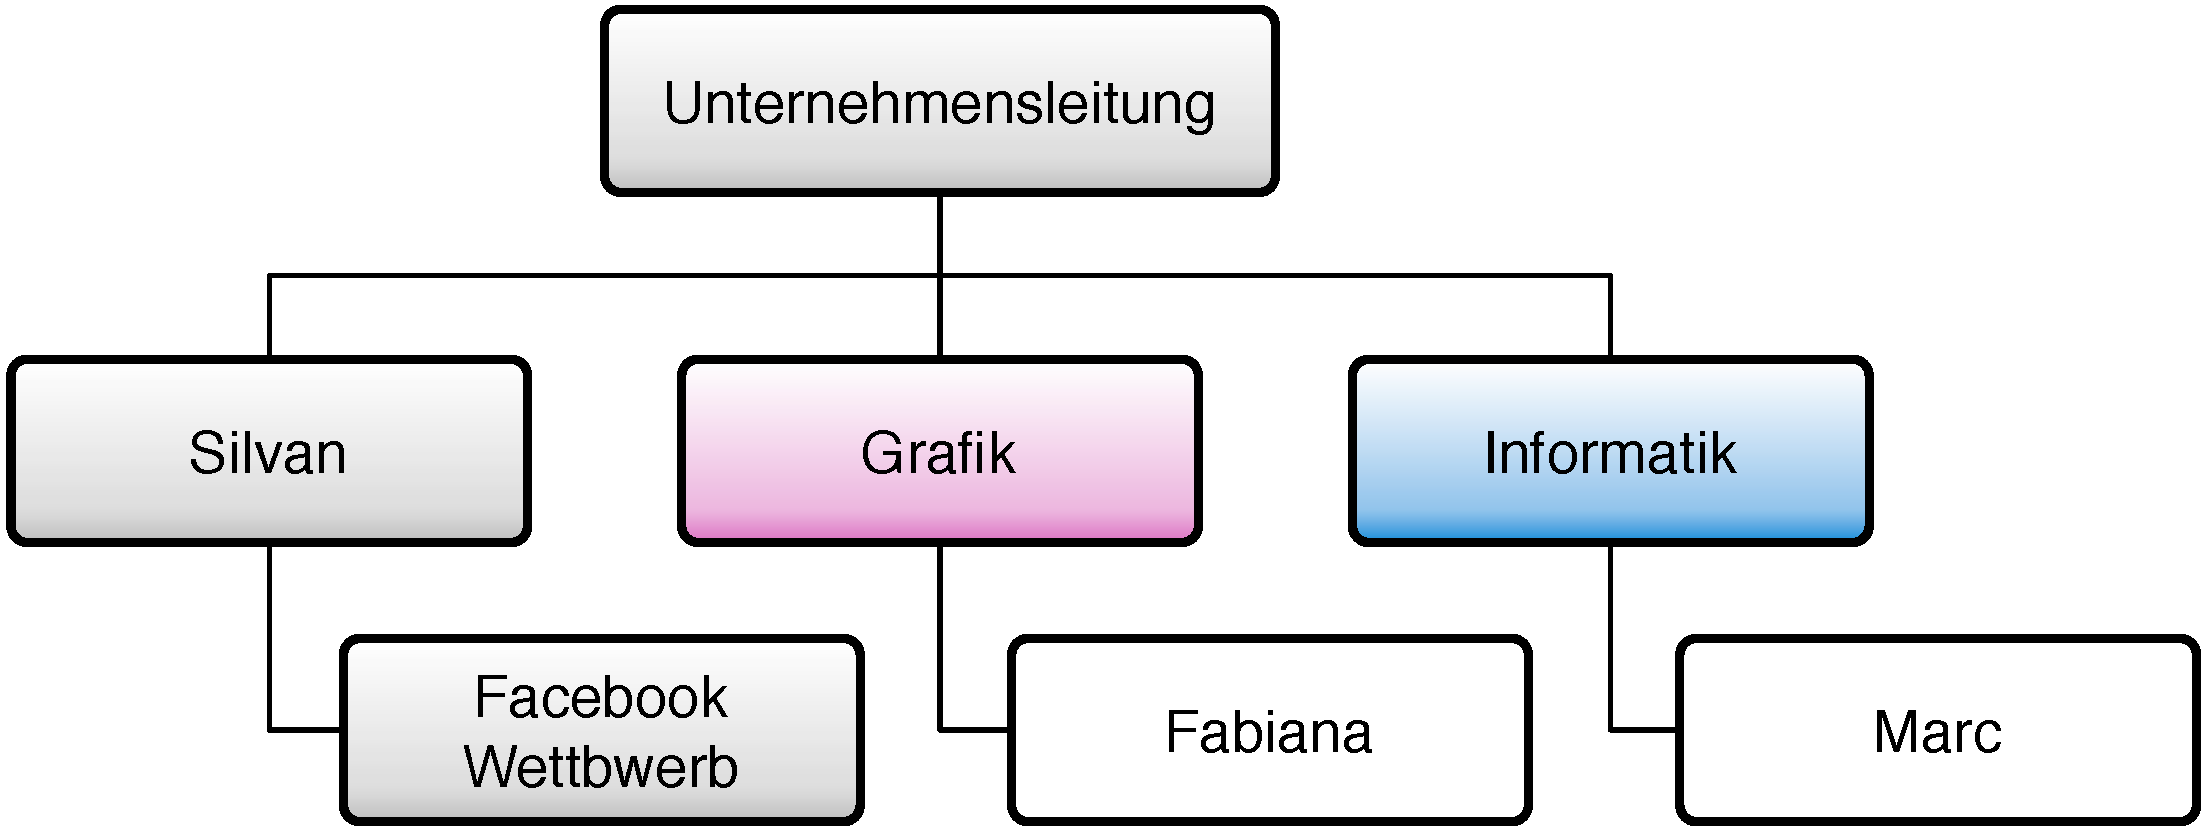
\includegraphics[width=0.7\textwidth,angle=0]{./bilder/proof_of_concept/projektorganisation_poc.pdf}
\caption[Projektorganisation Reisana Facebookwettbewerb]{Projektorganisation 
    Reisana Facebookwettbewerb\footnotemark}
\label{pic:projektorganisation_poc}
\end{center}
\end{figure}
\footnotetext{Eigene Darstellung}

Nachdem die Projektorganisation definiert ist, eröffnet der Projektleiter
im Projektmanagement Tool das Projekt. Die Projektdefinitionsphase ist somit 
abgeschlossen und das Projekt wechselt in die Projektplanungsphase.

\section{Projektplanung}
Als nächstes legt der Projektleiter die Datenablagestruktur auf dem Server an
und speichert alle Unterlagen des Kunden (\textbf{3.5}) in dem dafür vorgesehenen Ordner.
Eine Abbildung der Struktur ist in der Grafik \ref{pic:ablagestruktur_poc} ersichtlich.

\begin{figure}[htbp]
\begin{center}
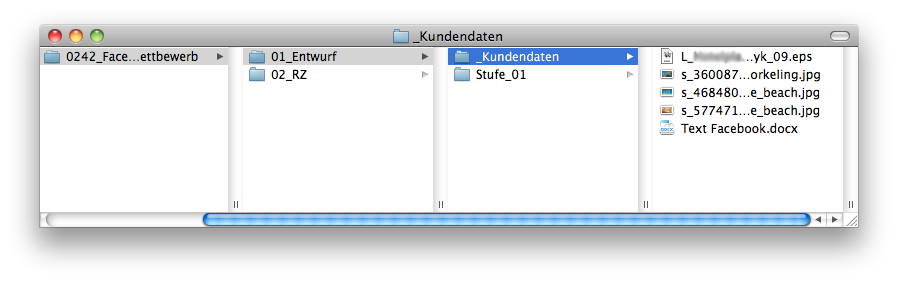
\includegraphics[width=1.0\textwidth,angle=0]{./bilder/proof_of_concept/ablagestruktur_poc.png}
\caption[Ablagestruktur des Facebook Wettbewerb Projektes]{Ablagestruktur des 
    Facebook Wettbewerb Projektes\footnotemark}
\label{pic:ablagestruktur_poc}
\end{center}
\end{figure}
\footnotetext{Eigene Darstellung}

Der Projektleiter erstellt nun in Zusammenarbeit mit seinem Projektteam die
zu erarbeiteten Arbeitspakete und erfasst diese im Projektmanagement Tool (\textbf{5.1}).
Zusammen werden die einzelnen Aufwände geschätzt (\textbf{5.2}), damit der 
Projektleiter die Offerte und Timings erstellen kann (\textbf{5.3}). In der
Abbildung \ref{pic:todos_poc} sieht man den Screenshot der geplanten Todos und die davon
abhängigen geplanten Meilensteine.

\begin{figure}[htbp]
\begin{center}
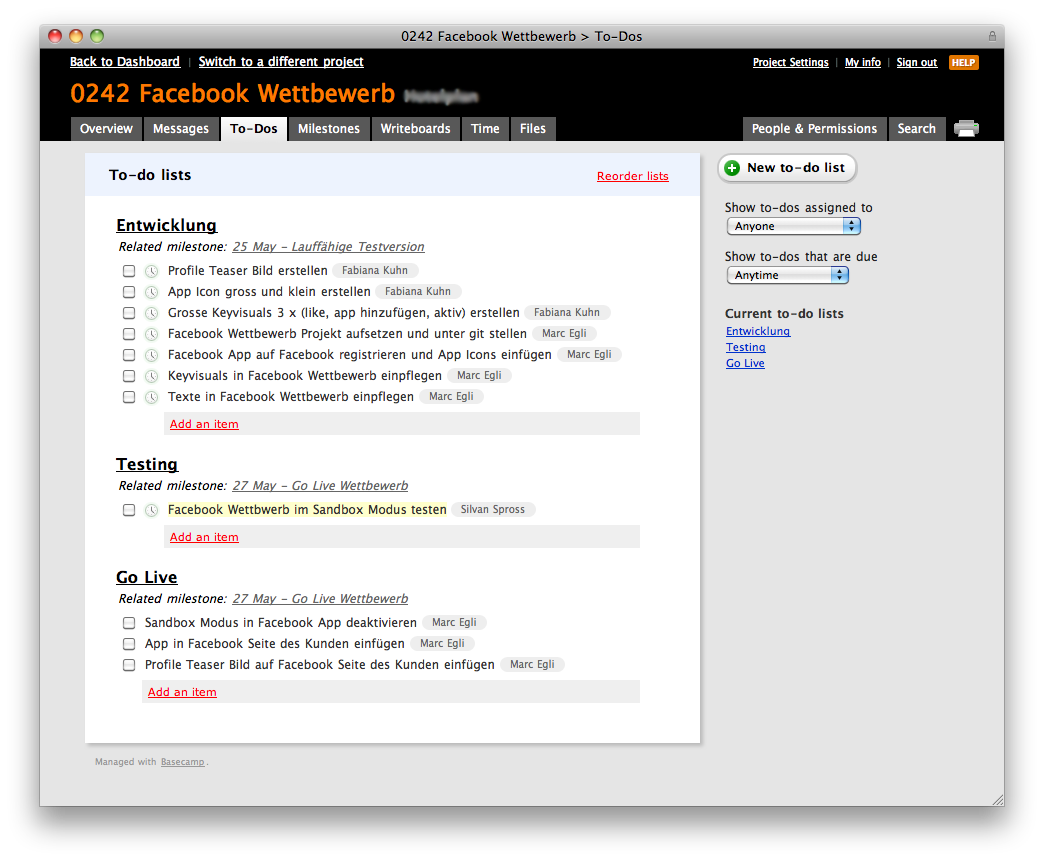
\includegraphics[width=1.0\textwidth,angle=0]{./bilder/proof_of_concept/todos_poc.png}
\caption[Die geplanten Todos mit den abhängigen Meilensteine des Projektes]{Die geplanten Todos 
    mit den abhängigen Meilensteine des Projektes\footnotemark}
\label{pic:todos_poc}
\end{center}
\end{figure}
\footnotetext{Screenshot aus Basecamp}

Als nächstes erstellt der Projektleiter die Offerte mit den geplanten Timings
(\textbf{5.3}). Da in diesem Fall der Projektleiter auch der verantwortliche
Partner ist (\textbf{5.4}) stellt dieser die Offerte auch gleich dem Kunden zu und bespricht
sie mit ihm (\textbf{5.6}).

Der Kunde hat die Offerte angenommen. Jetzt kann der Projektleiter in der 
Ressourcenplanung seine Mitarbeiter für das Projekt einplanen. In der nachfolgenden
Abbildung \ref{pic:ressourenplan_poc} sind die eingeplanten Stunden der Mitarbeiter
ersichtlich. Die geplanten Stunden basieren auf den Aufwandsschätzungen die im
Projektteam während der Erarbeitung der Arbeitspakete entstanden sind.

\begin{figure}[htbp]
\begin{center}
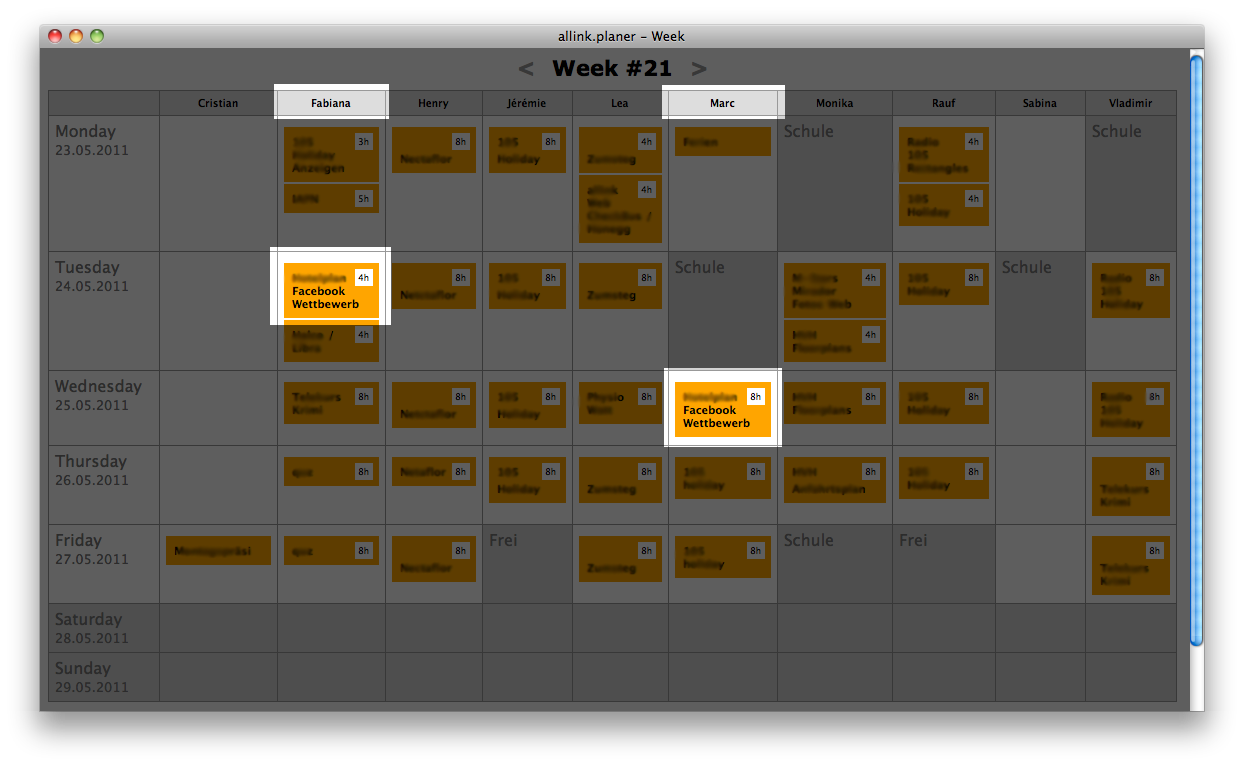
\includegraphics[width=1.0\textwidth,angle=0]{./bilder/proof_of_concept/ressourenplan_poc.png}
\caption[Ressourcenplanung des Projektes]{Ressourcenplanung des Projektes\footnotemark}
\label{pic:ressourenplan_poc}
\end{center}
\end{figure}
\footnotetext{Screenshot aus allink.planer}

Nun muss der Projektleiter noch die geplanten Geldflüsse im allink.planer erfassen, 
damit die Projektkennzahlen auch in die Liquiditätsplanung einfliessen. Dazu erfasst er
die Offerte und die geplanten Rechnungen. Wichtig ist die Wahl des Datums der 
geplanten Zahlung.

Das Projekt wird im allink.planer mit dem Basecamp Projekt verknüpft, damit später 
die rapportierten Stunden aus Basecamp bezogen werden können. Zudem wird auch gleich der Projektname
und die Projektnummer aus Basecamp importiert. In der Abbildung \ref{pic:geldfluessse_poc}
ist die Erfassung des Projektes im allink.planer ersichtlich.

\begin{figure}[htbp]
\begin{center}
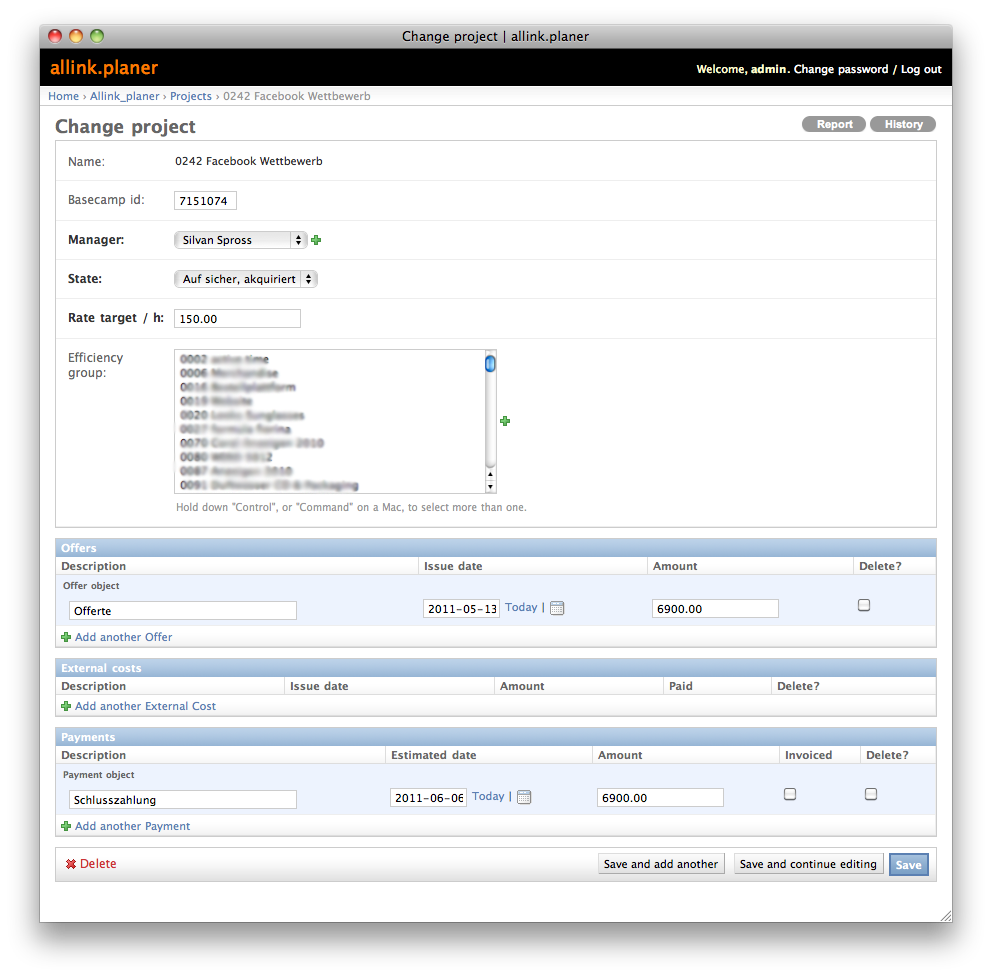
\includegraphics[width=1.0\textwidth,angle=0]{./bilder/proof_of_concept/geldfluessse_poc.png}
\caption[Die geplanten Geldflüsse des Projektes]{Die geplanten Geldflüsse des Projektes\footnotemark}
\label{pic:geldfluessse_poc}
\end{center}
\end{figure}
\footnotetext{Screenshot aus allink.planer}

Zu diesem Zeitpunkt sind alle Arbeitspakete, Ressourcen und Zahlungen geplant.
Somit wird mit der Umsetzung des Projektes begonnen und wir befinden uns in der
Phase der Projektkontrolle.

\section{Projektkontrolle}
Der Projektleiter kann nun laufend den Fortschritt des Projektes in Basecamp
verfolgen. Dank den Meilensteinen hat er stets den Überblick wann die damit
zusammenhängenden Todos abgeschlossen sein müssen. Die folgende Abbildung
\ref{pic:meilensteine_poc} zeigt die Meilensteinübersicht des Projektes in Basecamp.

\begin{figure}[htbp]
\begin{center}
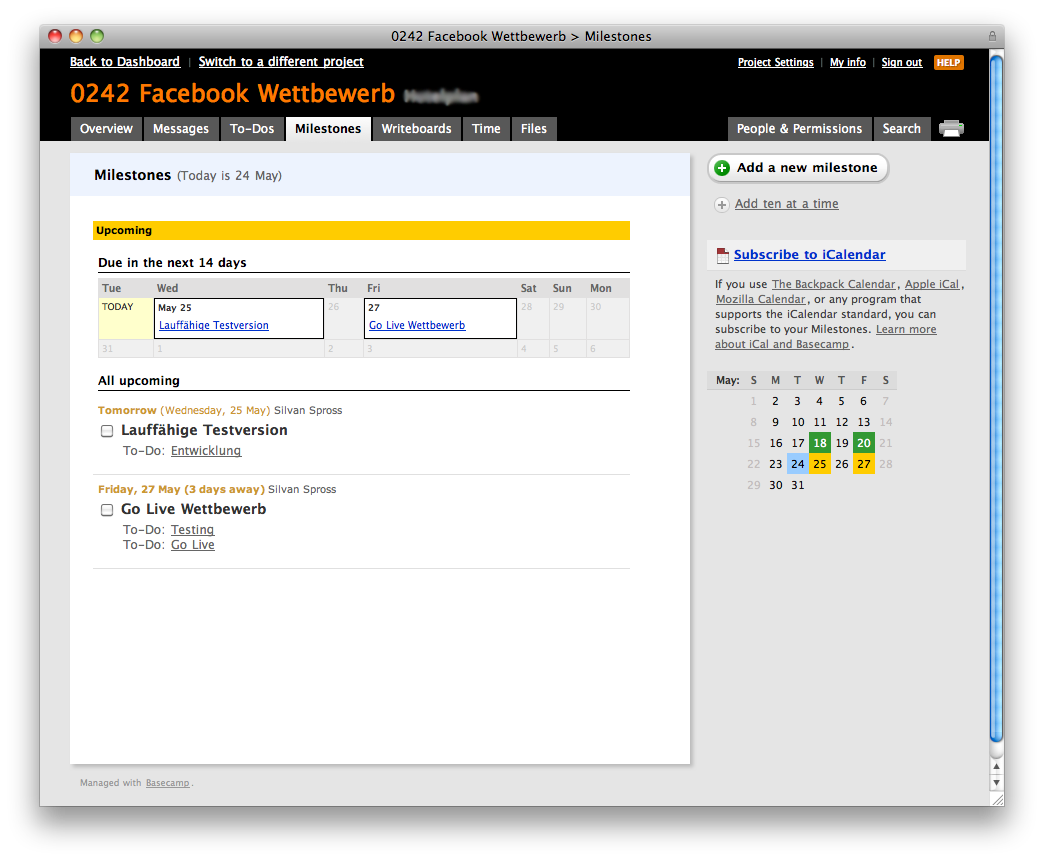
\includegraphics[width=1.0\textwidth,angle=0]{./bilder/proof_of_concept/meilensteine_poc.png}
\caption[Die geplanten Meilensteine mit den abhängigen Todolisten des Projektes]{Die 
    geplanten Meilensteine mit den abhängigen Todolisten des Projektes\footnotemark}
\label{pic:meilensteine_poc}
\end{center}
\end{figure}
\footnotetext{Screenshot aus Basecamp}

Die Mitarbeiter und natürlich auch der Projektleiter rapportieren laufend
ihre Stunden in Basecamp. Dank der Eigenentwicklung allink.timer können
diese sehr einfach erfasst werden. Die Abbildung \ref{pic:allink_timer} zeigt
ein Beispiel einer Zeitrapportierung.

\begin{figure}[htbp]
\begin{center}
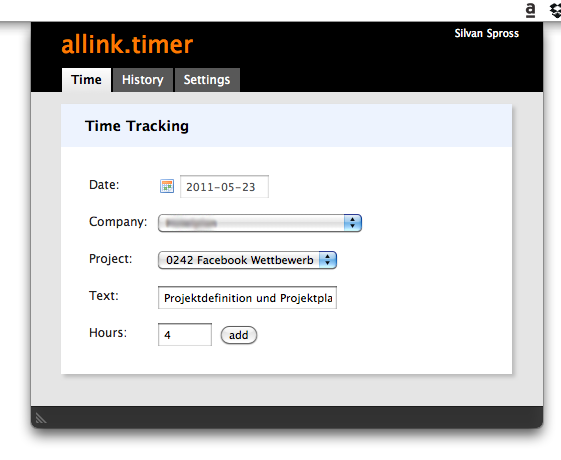
\includegraphics[width=0.7\textwidth,angle=0]{./bilder/proof_of_concept/allink_timer.png}
\caption[Beispiel einer Zeitrapportierung über allink.timer]{Beispiel einer 
    Zeitrapportierung über allink.timer\footnotemark}
\label{pic:allink_timer}
\end{center}
\end{figure}
\footnotetext{Screenshot aus allink.timer}

Wie man der Grafik entnehmen kann, muss der Mitarbeiter nur den Tag, die Firma
und das Projekt auswählen, danach kann er einen kurzen beschreibenden Text
zur getanen Arbeit und die Anzahl Stunden erfassen. Wie bereits erwähnt wird
die rapportierte Zeit in Basecamp gespeichert. Er hat zudem noch die Möglichkeit 
unter ``History'' die bereits erfassten Stunden pro Tag abzurufen. Somit kann 
er überprüfen, welche Arbeiten er heute oder an einem vergangen Tag schon rapportiert 
hat.

Das möglichst genaue Rapportieren ermöglicht dem Projektleiter und der Geschäftsleitung
ständigen einen Überblick über die finanzielle Lage des Projektes zu haben.
Im allink.planer kann pro Projekt ein aktueller Report angezeigt werden, der
die wichtigsten Kennzahlen des Projektes live berechnet. Die Abbildung \ref{pic:allink_planer_report}
zeigt den Report des Facebook Wettbewerb Projektes kurz nach der Projektplanungsphase.

\begin{figure}[htbp]
\begin{center}
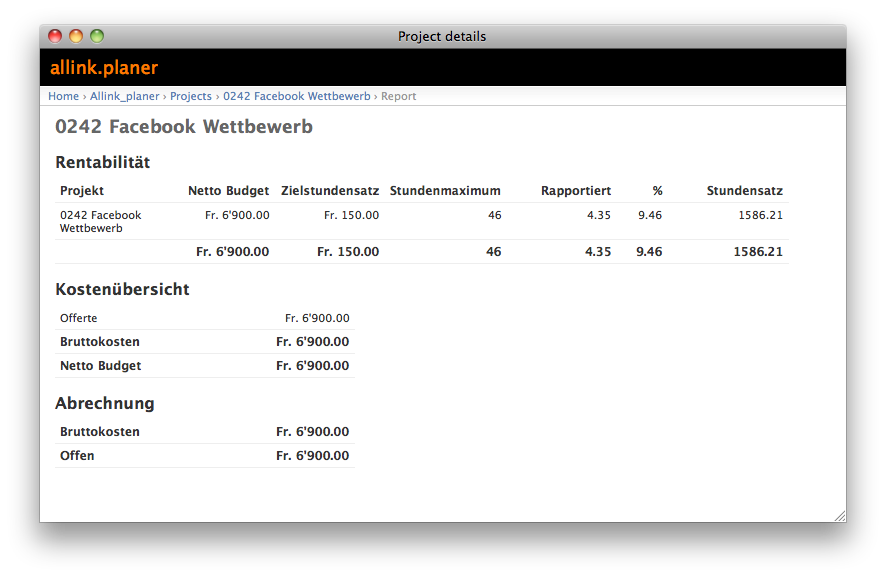
\includegraphics[width=1.0\textwidth,angle=0]{./bilder/proof_of_concept/allink_planer_report.png}
\caption[Report des Projektes kurz nach der Projektplanung]{Report des Projektes 
    kurz nach der Projektplanung\footnotemark}
\label{pic:allink_planer_report}
\end{center}
\end{figure}
\footnotetext{Screenshot aus allink.planer}

\clearpage

Alle diese projektspezifischen Daten fliessen in einem projektübergreifenden
Report zusammen, wo die Liquiditätsplanung vorgenommen werden kann. Auf diesen
haben zur Zeit nur die Partner von allink Zugriff. Die Abbildung \ref{pic:allink_planer_liq} stellt
diesen Report dar. Es wurden zusätzlich fiktive Projekte erfasst, damit der
Report möglichst realitätsnah dargestellt werden kann.

\begin{figure}[htbp]
\begin{center}
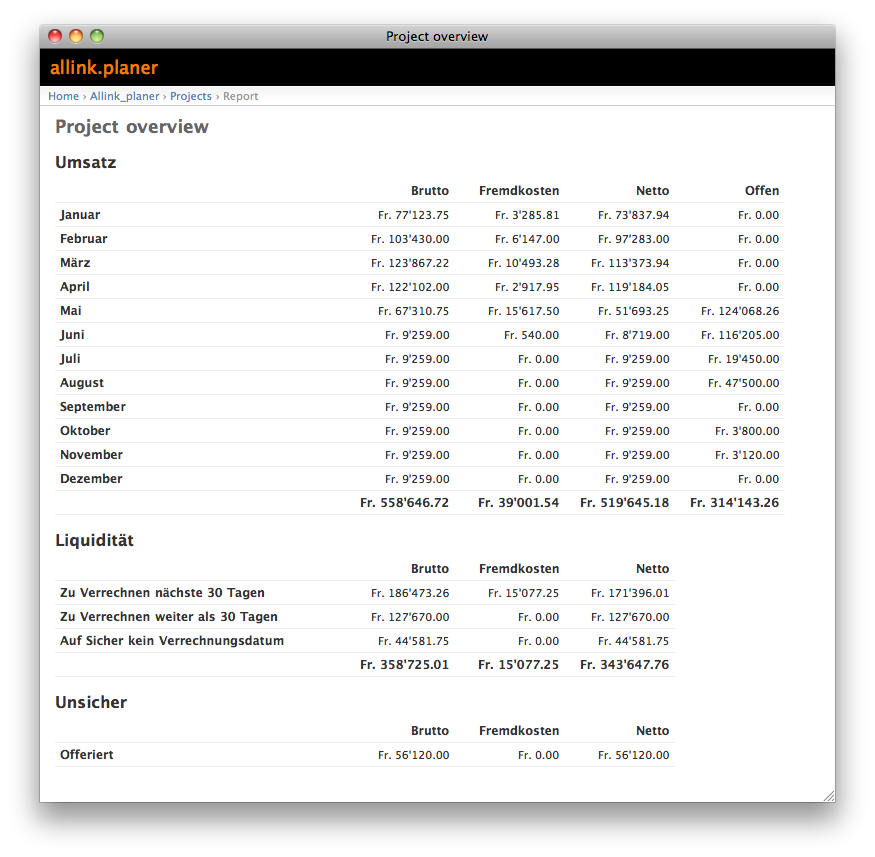
\includegraphics[width=1.0\textwidth,angle=0]{./bilder/proof_of_concept/allink_planer_liq.png}
\caption[Projektübergreifender Report zur Liquiditätsplanung]{Projektübergreifender 
    Report zur Liquiditätsplanung\footnotemark}
\label{pic:allink_planer_liq}
\end{center}
\end{figure}
\footnotetext{Screenshot aus allink.planer}

Somit ist sichergestellt, dass die Projektleiter und die Geschäftsführung eine
relativ genaue Termin- und Kostenkontrolle durchführen können.

\section{Projektabschluss}
Das Projekt wurde umgesetzt und die Todos der Realisierung sind abgearbeitet.
Nun folgt die Qualitätskontrolle (\textbf{7.2}) wofür der Projektleiter
verantwortlich ist und in diesem Fall auch gleich durchführt. Es wurden nur
kleine inhaltliche Mängel gefunden, die der Projektleiter selbst beheben
konnte (\textbf{7.3}). Es werden somit keine neuen Arbeitspakete definiert.

Der Projektleiter fasst nun die Resultate in einem Produktabnahmebericht 
zusammen (\textbf{9.1}). Da in diesem Projekt der Projektleiter auch gleich der 
verantwortliche Partner ist, geschieht dies in Form eines E-Mails, das direkt an 
die verantwortliche Person beim Kunden geschickt wird (\textbf{9.2}). Der Kunde 
kann nun die Testversion des Wettbewerbs online anschauen und begutachten (\textbf{9.3}).
Der Kunde hat sich daraufhin telefonisch mit dem Projektleiter in Verbindung
gesetzt und durchwegs positives Feedback zur Umsetzung abgegeben (\textbf{9.4}).
Auch hier wünscht der Kunde nur noch kleinere Anpassungen der Texte (\textbf{9.5}).
Da die Änderungen keine zusätzlichen Arbeitspakete benötigen, muss die Offerte
nicht angepasst werden. Nun folgen noch die letzten Todos um den Wettbewerb live 
zu schalten. Danach kann das Projekt abgeschlossen werden (\textbf{11.1}).
Der Projektleiter überprüft noch ein letztes mal den Projektreport, bevor er
das Projekt abschliesst und im allink.planer archiviert. Die Abbildung \ref{pic:allink_planer_report_ende}
zeigt den Report des Projektes kurz vor der Archivierung.

\begin{figure}[htbp]
\begin{center}
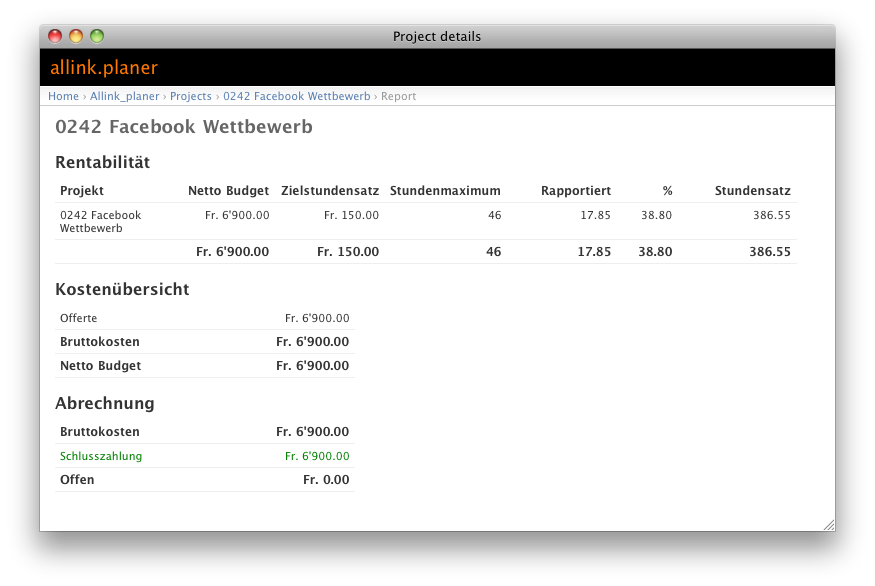
\includegraphics[width=0.87\textwidth,angle=0]{./bilder/proof_of_concept/allink_planer_report_ende.png}
\caption[Report des Projektes kurz vor der Archivierung]{Report des Projektes 
    kurz vor der Archivierung\footnotemark}
\label{pic:allink_planer_report_ende}
\end{center}
\end{figure}
\footnotetext{Screenshot aus allink.planer}

Wie man der Grafik entnehmen kann, war das Projekt sehr effizient. Es wurden knapp
über 55\% des geplanten Budgets aufgebraucht. Dabei muss jedoch beachtet werden,
dass das ganze Facebookwettbewerb Konzept bereits in zwei voran gegangenen Projekten
umgesetzt wurde und somit viel weniger Aufwand nötig war. Im ersten Projekt
wurde weit mehr als 100\% des damaligen Budgets aufgebraucht. Dank diesem
Projekt und hoffentlich noch weiteren Umsetzungen dieses Facebookwettbewerbs,
kann der damalige Aufwand quersubventioniert werden.

In der kurz gehaltenen Reflektionssitzung bei einem Kaffee wurden von den Mitarbeitern
und dem Projektleiter keine Probleme angesprochen. Das Projekt verlief für 
alle Beteiligten nahezu optimal.

\section{Anforderungsabdeckung}
Der Lösungsansatz scheint im ``Proof of Concept'' gut funktioniert zu haben.
Zum Abschluss wird noch überprüft ob auch im ``Proof of Concept'' alle 
Anforderungen abgedeckt werden konnten.

Dazu werden die im Kapitel \ref{chap:akzeptanzkriterien} definierten 
Akzeptanzkriterien erneut durchlaufen und geprüft. Dies ist in der nachfolgenden Tabelle 
\ref{tab:akzeptanzkriterien_test_poc} ersichtlich. Zur besseren Lesbarkeit wurde zur 
Akzeptanzkriteriumsnummer das Kriterium ein weiteres mal aufgelistet. Dazu wird 
der Status der Erfüllung gezeigt und in kurzen Worten beschrieben, wodurch das
Kriterium erfüllt wird.

\begin{longtable}{lp{6cm}p{5cm}l}
    \toprule \textbf{Nr.} & \textbf{Kriterium} & \textbf{Beschreibung} & \textbf{Status} \\
    \midrule AK1 &
        Wurde für das Projekt ein Hauptverantwortlicher Projektleiter definiert? &
        Ja, dies war Silvan Spross &
        erfüllt \\
    \midrule AK2 &
        Wurde für das Projekt ein Hauptverantwortlicher Partner definiert? &
        Ja, dies war ebenfalls Silvan Spross &
        erfüllt \\
    \midrule AK3 &
        Existiert für das Projekt ein Projektbrief? &
        Ja, wurde definiert. Vgl. Tabelle \ref{tab:projektbrief_poc} &
        erfüllt \\
    \midrule AK4 &
        Können für das Projekt Meilensteine und Arbeitspakete definiert werden? &
        Ja, wurden in Basecamp erfasst. Vlg. Abbildung \ref{pic:todos_poc} &
        erfüllt \\
    \midrule AK5 &
        Können die Mitarbeiter auf das Projekt Stunden rapportieren? &
        Ja, mit dem allink.timer. Vlg. Abbildung \ref{pic:allink_timer} &
        erfüllt \\
    \midrule AK6 &
        Sind die definierten Projektkennzahlen in einem System ersichtlich? &
        Ja, im allink.planer. Vlg. Abbildung \ref{pic:allink_planer_report}
        und \ref{pic:allink_planer_report_ende} &
        erfüllt \\
    \midrule AK7 &
        Sind die definierten Liquiditäts-Kennzahlen in einem System ersichtlich? &
        Ja, im allink.palner. Vgl. Abbildung \ref{pic:allink_planer_liq} &
        erfüllt \\
    \midrule AK8 &
        Existiert eine klare Struktur zur Ablage der Projektdaten? &
        Ja, auf dem allink Server. Vgl. Abbildung \ref{pic:ablagestruktur_poc} &
        erfüllt \\
    \midrule AK9 &
        Wurde für das Projekt ein Hauptverantwortlicher für die Qualitätssicherung definiert? &
        Ja, dies war Silvan Spross. &
        erfüllt \\
    \bottomrule
    \caption[Überprüfung der Akzeptanzkriterien im ``Proof of Concept'']{Überprüfung 
        der Akzeptanzkriterien im ``Proof of Concept''\footnotemark}
    \label{tab:akzeptanzkriterien_test_poc}
\end{longtable}
\footnotetext{Eigene Darstellung}

Im ``Proof of Concept'' wurden ebenfalls alle Akzeptanzkriterien erfüllt
und somit alle definierten Anforderungen abgedeckt. Das bestätigt, dass der
Lösungsansatz funktioniert und so definitiv umgesetzt werden kann.
